\documentclass[border=3mm]{standalone}
\usepackage{fontspec,xeCJK,graphicx,tikz,amsmath,amssymb}
\setmainfont{Helvetica}\setCJKmainfont{PingFang SC}
\usetikzlibrary{arrows.meta,positioning}
\definecolor{ink}{HTML}{173347}\definecolor{teal}{HTML}{217F83}\definecolor{amber}{HTML}{B96316}\definecolor{paper}{HTML}{FCFAF5}\definecolor{bluefill}{HTML}{EAF3F7}\definecolor{greenfill}{HTML}{E7F3EF}\definecolor{goldfill}{HTML}{FCEDDA}
% Scientific source: arXiv 2609.35709v1, §§3.1–3.4,4.5, Eqs1–14, Tables1,6.
% Image material is reused unchanged from the actual built-in imagegen draft.
% The EEF48 task-space representation is explicitly for shared training (§3.1).
\begin{document}
\begin{tikzpicture}[x=1cm,y=1cm,>=Latex,text=ink,
 txt/.style={align=center,font=\fontsize{14}{18}\selectfont},
 head/.style={align=left,font=\fontsize{17}{22}\selectfont\bfseries},
 panel/.style={rounded corners=2mm,draw=teal!50,fill=bluefill,line width=.8pt},
 cell/.style={rounded corners=2mm,draw=teal!55,fill=white,align=center,font=\fontsize{14}{18}\selectfont},
 flow/.style={->,line width=1.2pt,draw=teal},
 teach/.style={->,dashed,line width=1.2pt,draw=amber}]
\path[fill=paper] (-6.7,.1) rectangle (6.7,-42.9);
\node[inner sep=0,anchor=north] at (0,0) {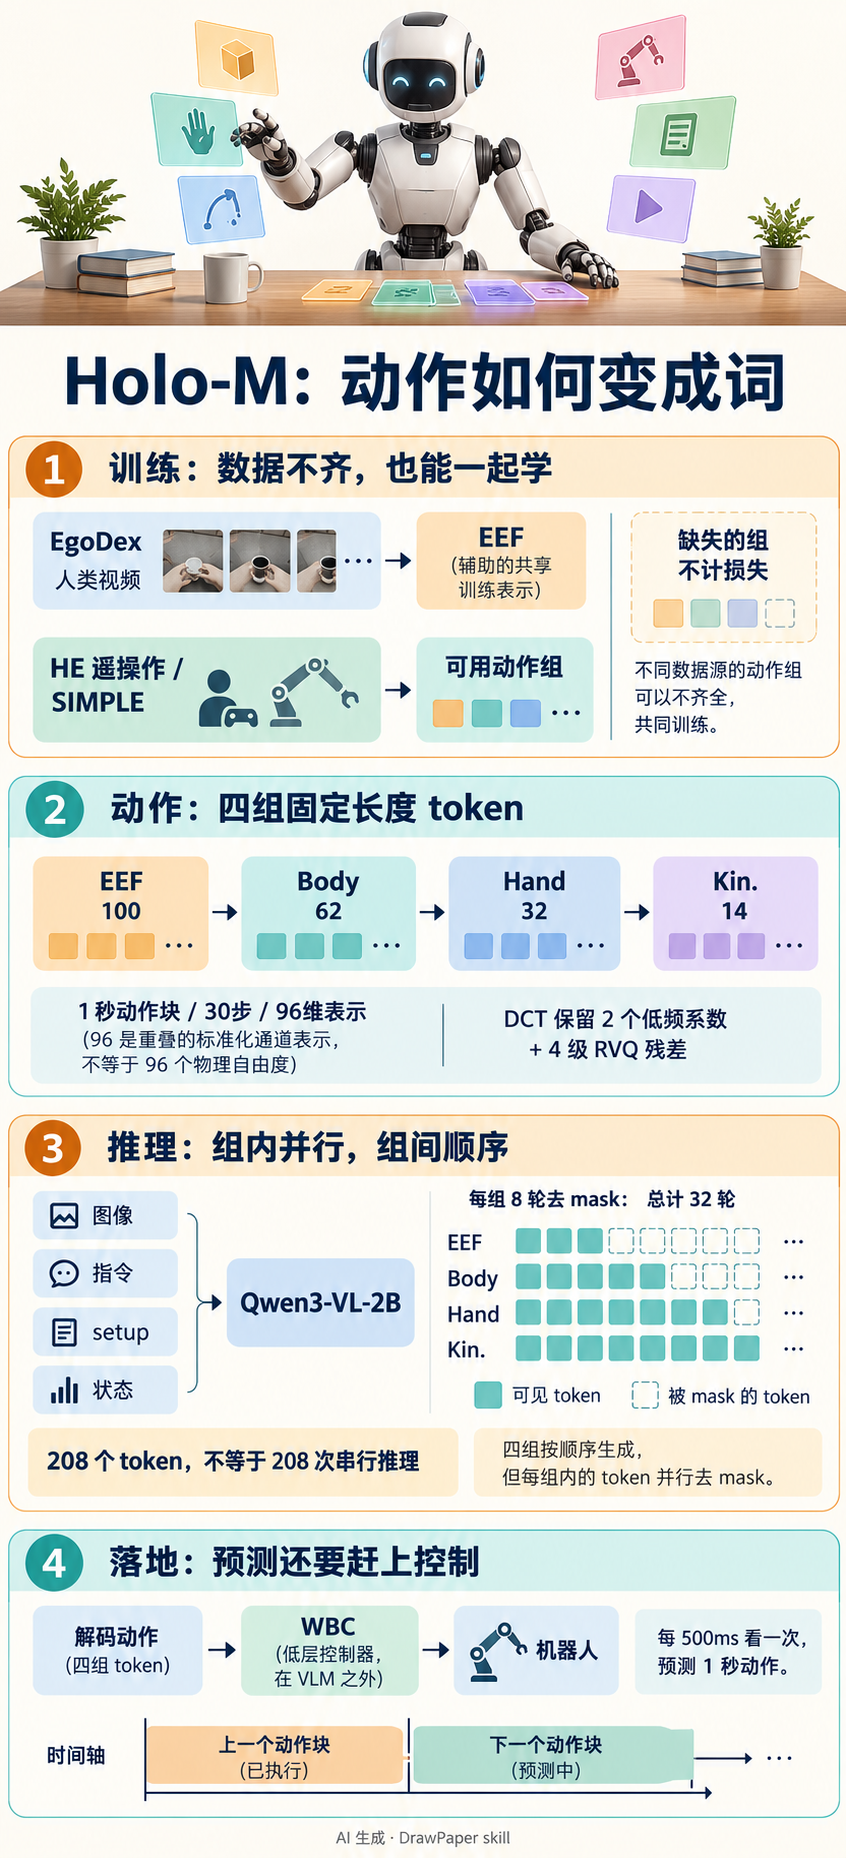
\includegraphics[viewport=0 1532 846 1858,clip,width=12.4cm]{holo-m-imagegen-draft.png}};
\node[head,align=center] at (0,-5.05) {Holo-M：训练与执行全图};
\node[txt] at (0,-5.85) {训练：A $\to$ B $\to$ E，E 更新 D\\运行：C $\to$ D $\to$ F，现场反馈回 C};
\draw[panel,fill=goldfill,draw=amber!60] (-6.2,-6.6) rectangle (6.2,-9.45);
\node[head,anchor=west,text=amber] at (-5.9,-7.18) {A｜示范数据与可用标签};
\node[txt] at (0,-8.15) {EgoDex：人类手部视频，监督 EEF\\Humanoid Everyday / SIMPLE：可用动作组};
\node[txt] at (0,-9.0) {一秒动作块：$30\times96$；缺失组开关为 0};
\draw[teach] (0,-9.48)--(0,-9.95);
\draw[panel] (-6.2,-10) rectangle (6.2,-16.1);
\node[head,anchor=west] at (-5.9,-10.55) {B｜FAST-RVQ：连续轨迹 $\to$ 编号};
\node[txt] at (0,-11.4) {四组宽度：EEF 48 / Body 29 / Hand 14 / Kin. 5\\每组输入 $X_g\in\mathbb R^{30\times D_g}$};
\node[cell,minimum width=11.5cm,minimum height=1.35cm] (dct) at (0,-12.65) {时间 DCT $\to$ 每维保留 2 个低频系数\\低频量化：$2D_g$ 个 token；逆 DCT 得平滑轨迹};
\node[cell,minimum width=11.5cm,minimum height=1.35cm] (rvq) at (0,-14.35) {原轨迹 $-$ 平滑轨迹 $=$ 整组时域残差\\4 级 RVQ：逐级找码向量、减误差 $\to$ 4 个编号};
\draw[flow] (dct.south)--(rvq.north);
\node[txt] at (0,-15.6) {$L_g=2D_g+4$；四组长度 100 / 62 / 32 / 14\\输出：208 个目标动作 token（边界另计）};
\draw[teach] (0,-16.13)--(0,-16.55);
\draw[panel,fill=goldfill,draw=amber!60] (-6.2,-16.6) rectangle (6.2,-22.65);
\node[head,anchor=west,text=amber] at (-5.9,-17.15) {E｜训练：只对有标签的组批改};
\node[txt] at (0,-18.25) {输入：B 的目标编号 + C 的观测条件\\$v_g$ 标签开关；$w_g$ 组权重};
\node[txt] at (0,-19.3) {AR：按全部有效 token 数平均\\分组恢复：先组内平均，再按组权重混合};
\node[txt] at (0,-21.15) {混合数据 AR $\to$ SIMPLE AR $\to$ 分组恢复\\可选：单任务专才\\更新语言骨干；视觉编码器冻结};
\draw[panel,fill=greenfill] (-6.2,-23.15) rectangle (6.2,-27.65);
\node[head,anchor=west,text=teal] at (-5.9,-23.7) {C｜当前观测 $\to$ 多模态上下文};
\node[cell,minimum width=11.5cm,minimum height=1.25cm] (vision) at (0,-24.75) {RGB $640\times360$ $\to$ 视觉编码器 $\to$ 视觉特征\\任务文字 + setup 本体/来源标识};
\node[cell,minimum width=11.5cm,minimum height=1.3cm] (state) at (0,-26.4) {实机 31 个上半身角度 $\to$ 裁剪 / 归一化\\每角度选一个 256 档状态 token $\to$ 拼接上下文 $c_t$};
\draw[flow] (vision.south)--(state.north);
\draw[flow] (0,-27.68)--(0,-28.1);
\draw[panel,fill=greenfill] (-6.2,-28.15) rectangle (6.2,-33.8);
\node[head,anchor=west,text=teal] at (-5.9,-28.7) {D｜Qwen3-VL-2B：分组恢复动作};
\node[txt] at (0,-29.58) {同一扩展词表；输入 $c_t$ + 已完成组\\当前组全 [MASK] $\to$ 并行提案 $\to$ 高置信位置保留};
\foreach \xx/\lab/\num in {-4.5/EEF/100,-1.5/Body/62,1.5/Hand/32,4.5/Kin./14}{\node[cell,minimum width=2.5cm,minimum height=1.0cm] at (\xx,-31.05) {\lab\\\num};}
\foreach \xx in {-3,0,3}{\draw[flow] (\xx-.19,-31.05)--(\xx+.19,-31.05);}
\node[txt] at (0,-32.42) {组内双向看；跨组沿 EEF $\to$ Body $\to$ Hand $\to$ Kin.\\每组 8 轮，共 32 轮；前缀 / 已完成组缓存};
\node[txt] at (0,-33.4) {输出：208 个动作编号};
% Supervision/update remains outside panels. No line crosses explanatory text.
\draw[teach] (-6.22,-21.6)--(-6.5,-21.6)--(-6.5,-30.1)--(-6.22,-30.1);
\draw[flow] (0,-33.83)--(0,-34.25);
\draw[panel] (-6.2,-34.3) rectangle (6.2,-42.0);
\node[head,anchor=west] at (-5.9,-34.85) {F｜编号还原 $\to$ WBC $\to$ 机器人};
\node[cell,minimum width=11.5cm,minimum height=1.4cm] (inverse) at (0,-36.55) {低频编号查系数 $\to$ 逆 DCT；残差编号查码向量\\相加还原 $30\times D_g$ 轨迹\\EEF：共享训练表征；关节 / 底座目标进入控制链};
\node[cell,minimum width=11.5cm,minimum height=1.0cm] (wbc) at (0,-38.25) {WBC 跟踪高层目标\\下肢强化学习控制 + 上肢 IK $\to$ 机器人动作};
\draw[flow] (inverse.south)--(wbc.north);
\node[txt] at (0,-39.65) {每 500 ms 观测；每块预测 1 秒 / 30 步\\旧块执行与新块推理交叠；新块跳过 hold 内前段};
\node[txt] at (0,-40.9) {首块立即执行；8 轮 hold 为 500 ms\\新块从第 15 步接管；现场画面 / 状态反馈回 C};
\draw[flow] (6.22,-38.1)--(6.5,-38.1)--(6.5,-24.75)--(6.22,-24.75);
\node[txt,font=\fontsize{12}{16}\selectfont] at (0,-42.55) {实线：计算 / 运行反馈　虚线：监督 / 参数更新};
\end{tikzpicture}
\end{document}
